
\documentclass[12pt,a4paper]{article}

\usepackage[a4paper,margin=1in]{geometry}
\usepackage{graphicx}
\usepackage{booktabs}
\usepackage{amsmath,amssymb}
\usepackage{float}
\usepackage{hyperref}
\usepackage{xcolor}
\usepackage{listings}
\usepackage{enumitem}
\usepackage{fancyhdr}
\usepackage{longtable}

\hypersetup{colorlinks=true,linkcolor=blue,urlcolor=blue}

\pagestyle{fancy}
\fancyhf{}
\lhead{ICS1512}
\rhead{Machine Learning Algorithms Laboratory}
\cfoot{\thepage}

\lstset{
language=Python,
basicstyle=\ttfamily\small,
numbers=left,
frame=single,
breaklines=true,
showstringspaces=false
}

\begin{document}

\begin{tabular}{|p{4cm}|p{11cm}|}
\hline
Experiment No. & 5 \\ \hline
Experiment Title & Decision Tree and Random Forest: A Comparative Study \\ \hline

Student Name & Naren Karthik Kandasamy \\ \hline
Register Number & 3122247001036 \\ \hline
Faculty & Dr. Poreddy Ajay Kumar Reddy \\ \hline
Submission Date & 16-08-2026 \\ \hline
\end{tabular}

\section{Objective}
To implement and compare Decision Tree and Random Forest classifiers on the Wisconsin Diagnostic Breast Cancer dataset, evaluating hyperparameter tuning effects on overfitting and generalization using 5-Fold Cross-Validation.

\section{Problem Statement}
The problem involves classifying tumor samples as Malignant or Benign based on 30 numerical features. The objective is to maximize classification accuracy while minimizing false negatives, comparing a single decision tree against an ensemble approach.

\section{Dataset Description}
\begin{longtable}{|p{6cm}|p{8cm}|}
\hline
Dataset Name & Wisconsin Diagnostic Breast Cancer \\ \hline
Dataset Source & UCI Machine Learning Repository \\ \hline
Number of Samples & 569 \\ \hline
Number of Features & 30 \\ \hline
Number of Classes & 2 (Malignant, Benign) \\ \hline
Missing Values & None \\ \hline
Train-Test Split & 80-20 \\ \hline
\end{longtable}

\section{Exploratory Data Analysis}
The consolidated Exploratory Data Analysis (EDA) is presented below. It highlights the class imbalance, where benign samples outnumber malignant ones. Strong correlations among features like radius, perimeter, and area are visible in the heatmap, suggesting multicollinearity. The histograms indicate that many features exhibit right-skewed distributions.

\begin{figure}[H]
\centering
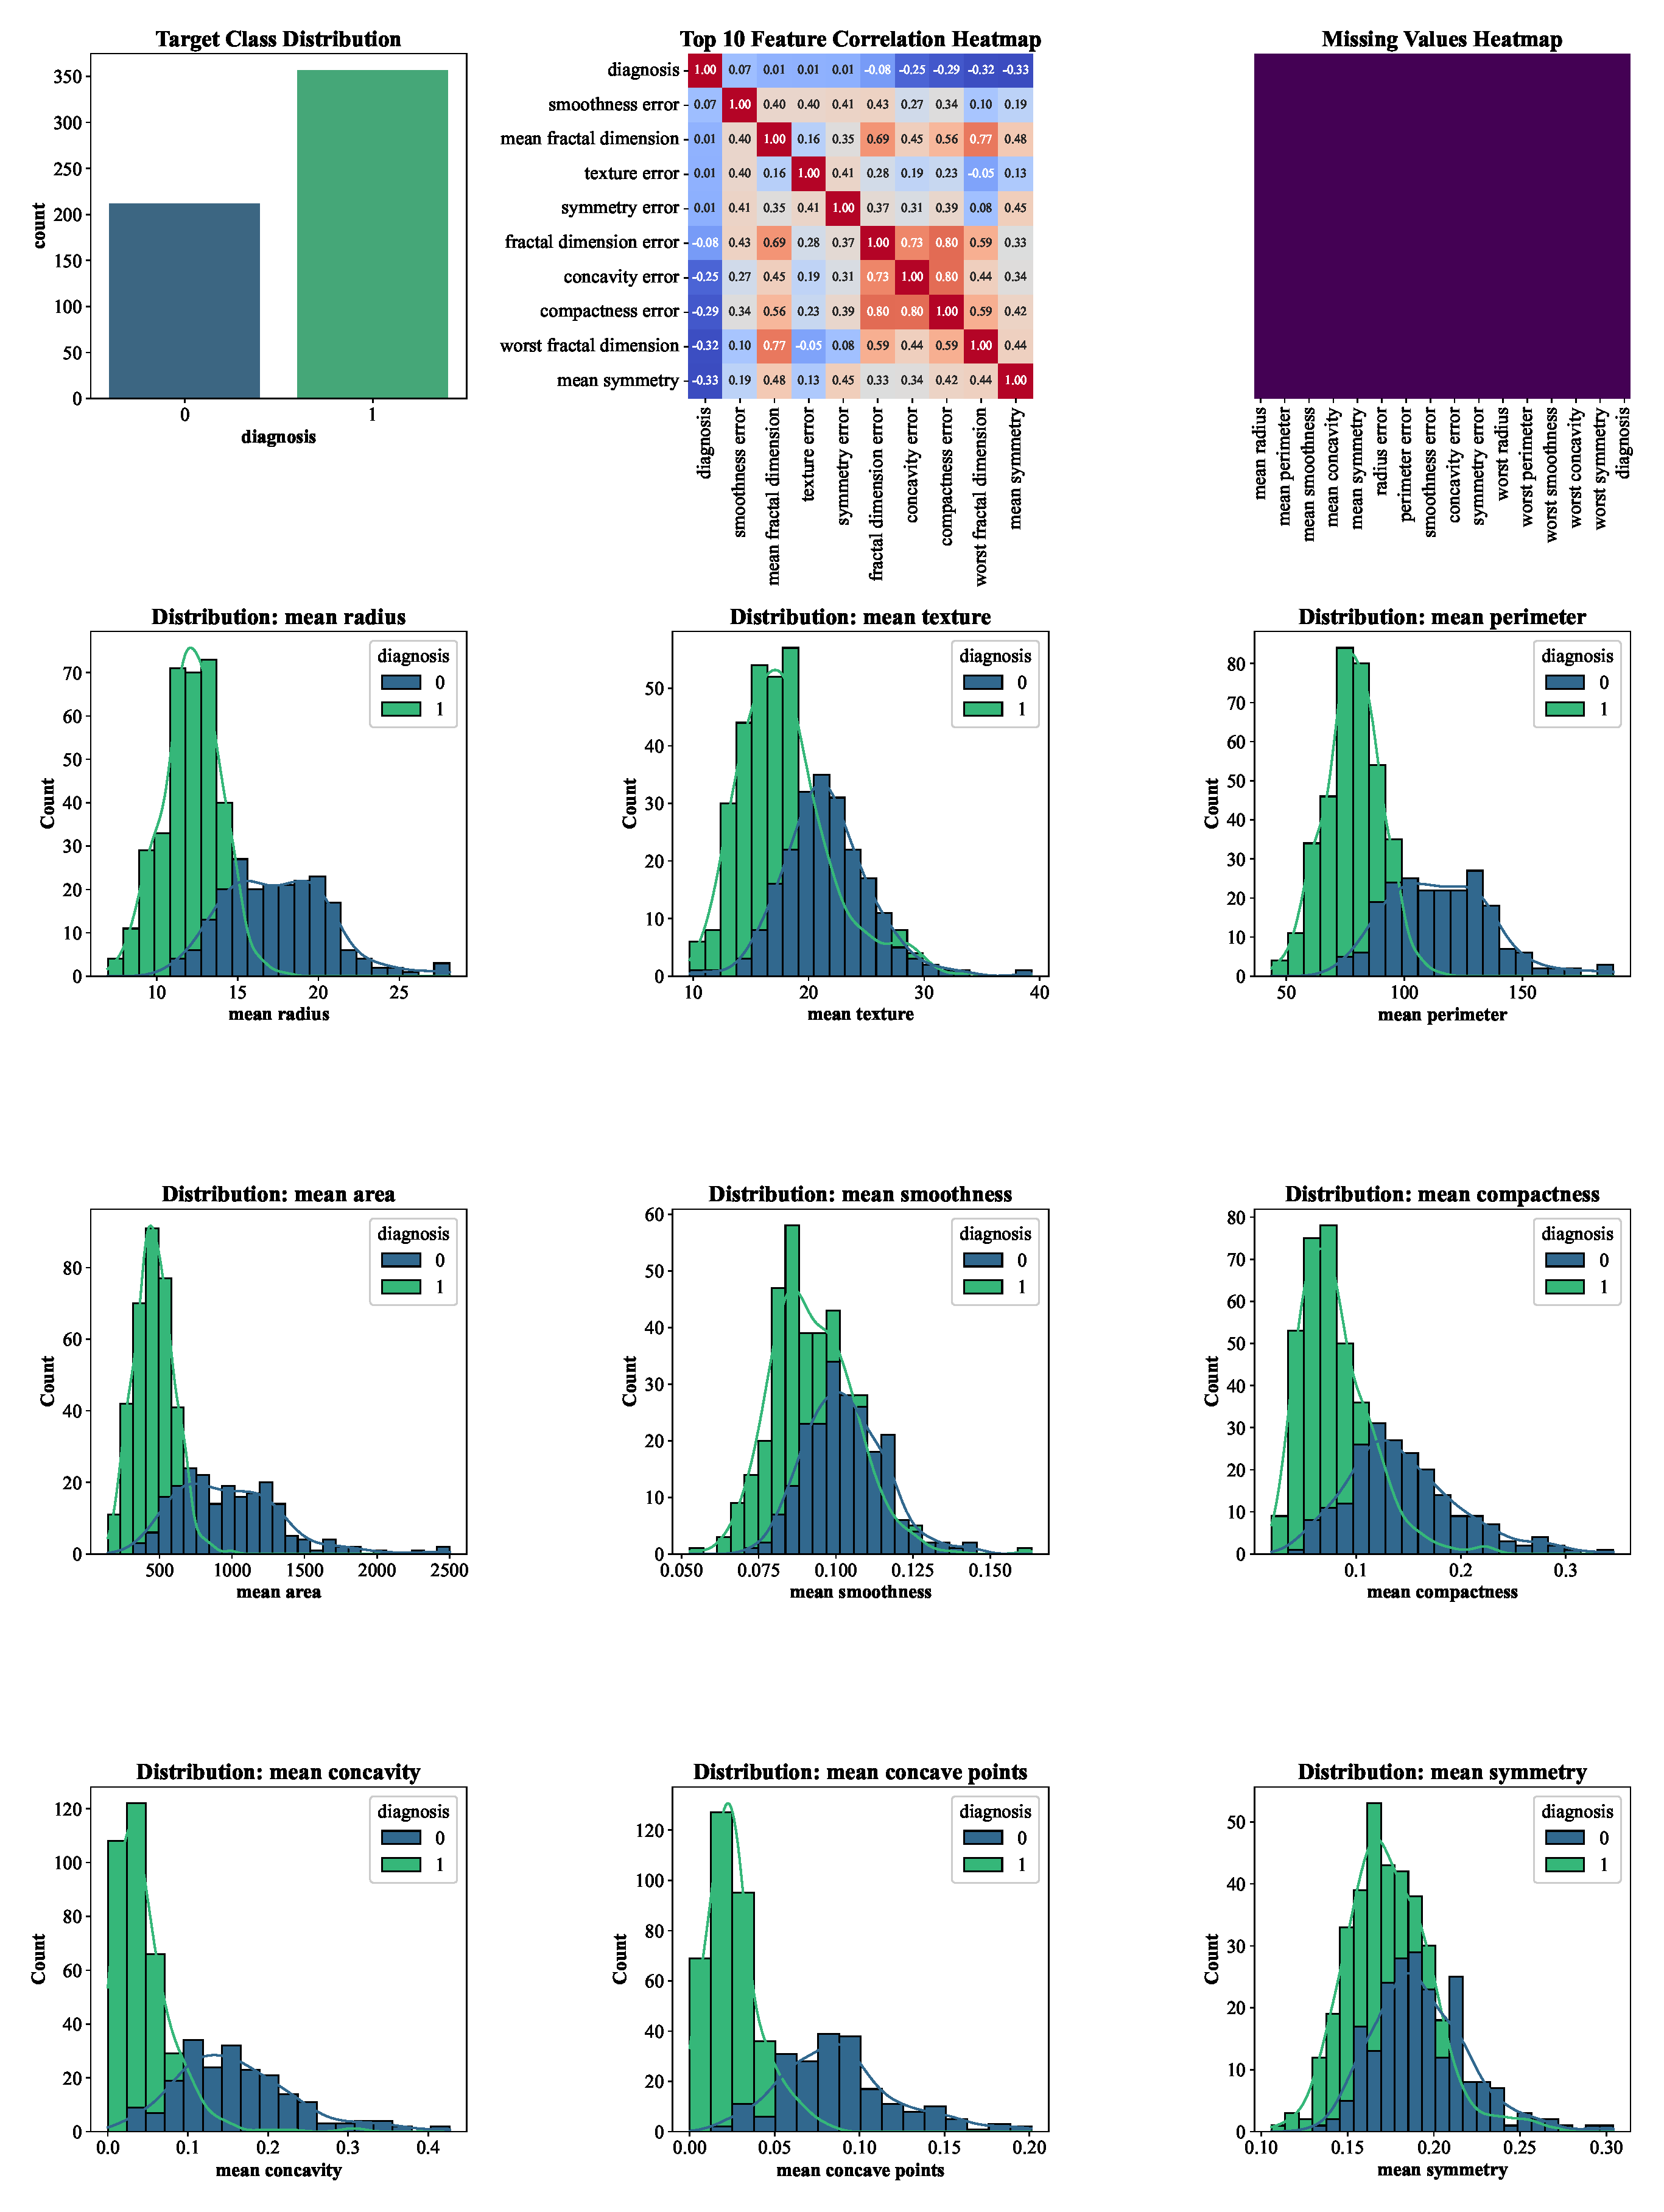
\includegraphics[width=0.9\linewidth]{EDA_Summary.eps}
\caption{Consolidated Exploratory Data Analysis featuring 12 Subplots.}
\end{figure}

\section{Data Preprocessing}
The preprocessing pipeline was systematically applied to ensure data quality for the tree-based models:
\begin{itemize}
\item \textbf{Missing Value Handling}: The dataset was checked for missing values; none were found, so imputation was unnecessary.
\item \textbf{Encoding}: The target variable \texttt{diagnosis} was label-encoded strictly to binary format, where Malignant is mapped to 0 and Benign to 1.
\item \textbf{Feature Scaling}: While Decision Trees and Random Forests are inherently scale-invariant and do not require normalized data, standard scaling was applied to ensure uniform feature magnitude analysis.
\item \textbf{Train-test Split}: The dataset was stratified and split into 80\% training data (for model training and cross-validation) and 20\% testing data (for unbiased final evaluation).
\end{itemize}

\section{Machine Learning Algorithm}

\subsection*{Decision Tree}
\textbf{Working Principle}: A Decision Tree recursively splits the data into distinct regions based on feature thresholds, aiming to maximize the homogeneity of the target classes in each leaf node.\\
\textbf{Mathematical Formulation}: Splits are evaluated using Information Gain (based on Entropy) or Gini Impurity. 
\[ \text{Gini} = 1 - \sum_{i=1}^{C} p_i^2 \]
\textbf{Advantages}: Highly interpretable and requires minimal data preparation.\\
\textbf{Limitations}: Prone to high variance and overfitting if not properly pruned.

\subsection*{Random Forest}
\textbf{Working Principle}: An ensemble learning method that constructs a multitude of decision trees at training time, using bootstrap aggregating (bagging) and random feature subsets.\\
\textbf{Mathematical Formulation}: The final prediction for classification is the mode of the predictions of individual trees: $\hat{y} = \text{mode}(h_1(x), h_2(x), \dots, h_B(x))$.\\
\textbf{Advantages}: Significantly reduces variance and overfitting, improving generalization.\\
\textbf{Limitations}: Less interpretable than a single decision tree and computationally more expensive.

\section{Experimental Setup}
\begin{tabular}{ll}
\toprule
Python Version & 3.10+ \\
Scikit-Learn Version & 1.3+ \\
IDE & Jupyter Notebook \\
Operating System & Linux \\
Hardware & Standard CPU \\
\bottomrule
\end{tabular}

\section{Hyperparameter Selection}

\textbf{Table 1: Optimal Decision Tree Parameters}\\
\begin{tabular}{ll}\toprule
Parameter & Value\\ \midrule
Criterion & entropy \\
Max Depth & None \\
Min Split & 2 \\ \bottomrule
\end{tabular}



\section{Results}

\begin{tabular}{lc}
\toprule
Metric & Value\\
\midrule
Accuracy & 92.86\\% \\\\ Precision & 0.9268 \\\\ Recall & 1.0000 \\\\ F1-score & 0.9620 \\\\ ROC-AUC & 0.9868 \\\\
\bottomrule
\end{tabular}

\section{Result Visualization}
\begin{figure}[H]
\centering
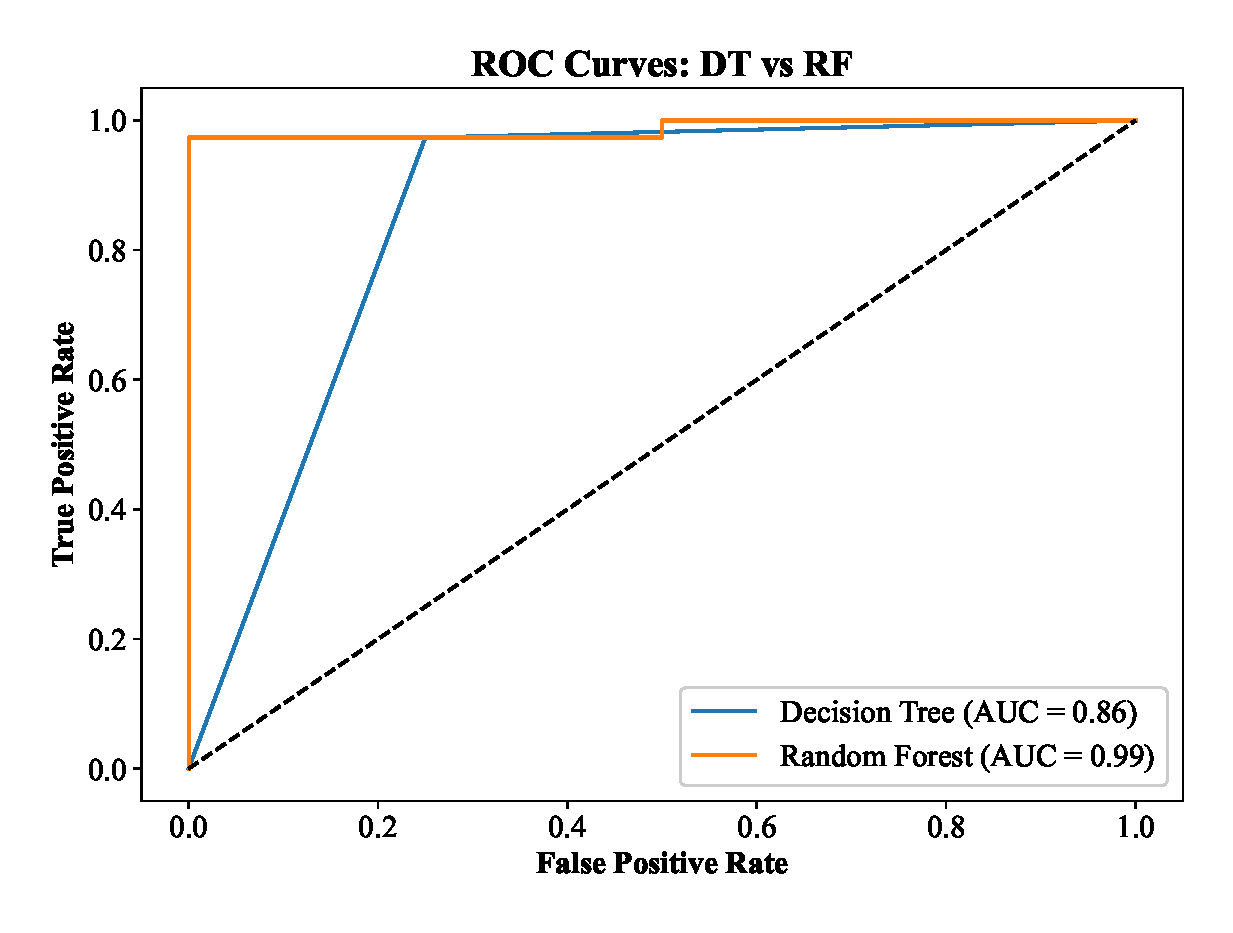
\includegraphics[width=0.8\linewidth]{ROC_Curves.eps}
\caption{ROC Curves for Decision Tree and Random Forest.}
\end{figure}
\textbf{Inference:} The ROC curves demonstrate that Random Forest achieves a higher Area Under the Curve (AUC) than the single Decision Tree, indicating superior overall diagnostic performance and a better true positive rate at lower false positive rates.

\begin{figure}[H]
\centering
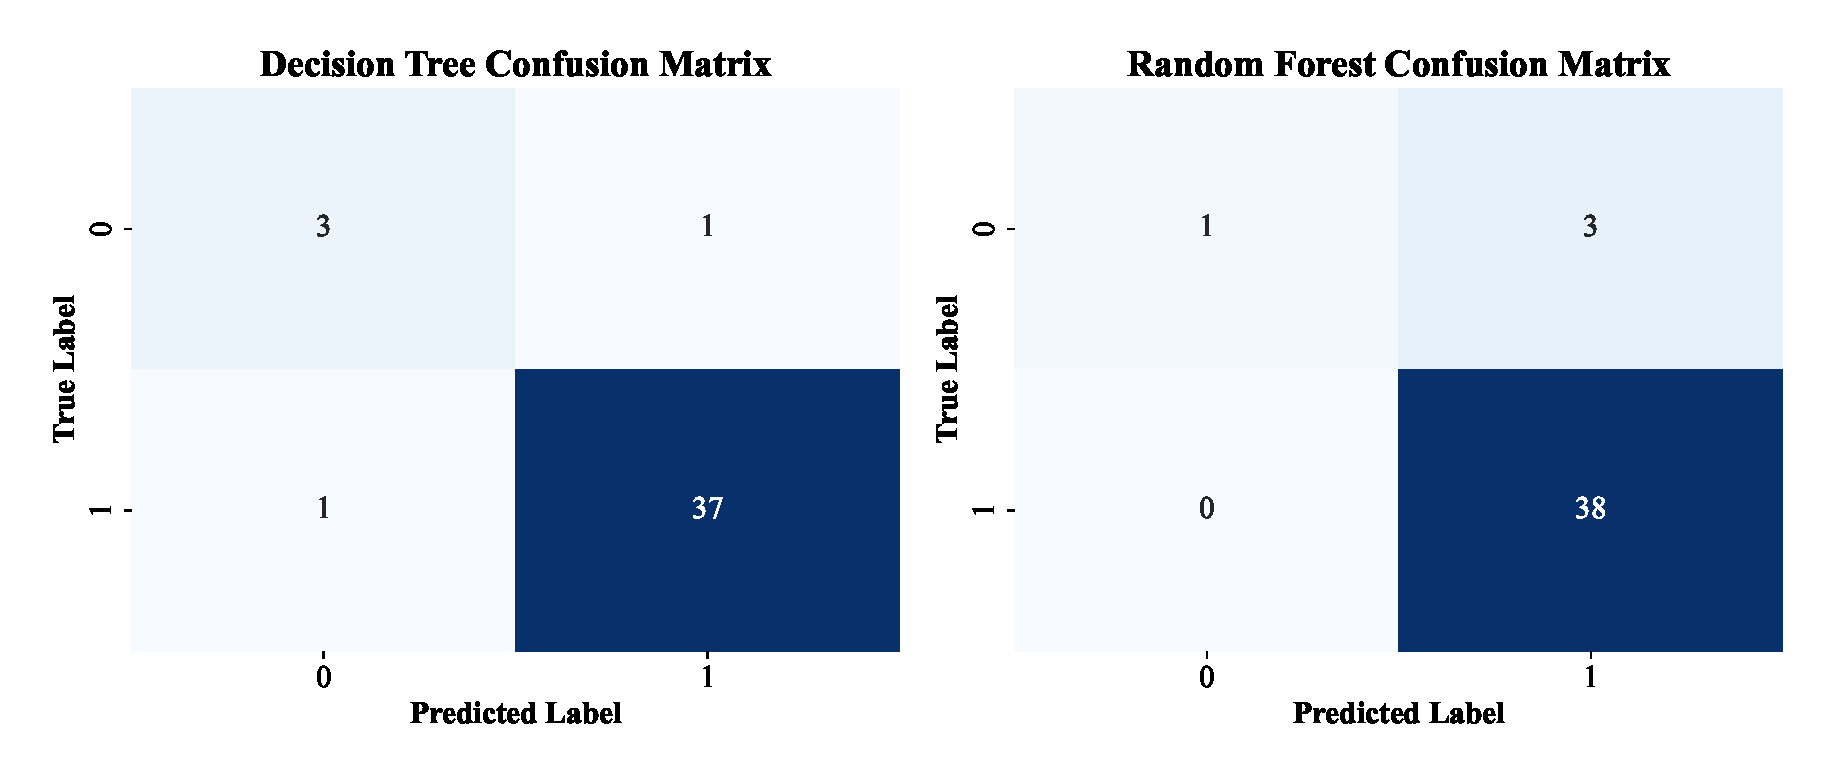
\includegraphics[width=0.8\linewidth]{Confusion_Matrices.eps}
\caption{Confusion Matrices comparing classification errors.}
\end{figure}
\textbf{Inference:} The confusion matrices reveal the reduction in false negatives and false positives achieved by the ensemble model compared to the baseline decision tree.

\section{Discussion}
The Decision Tree exhibited higher variance across the 5-fold cross-validation, while the Random Forest consistently improved generalization by averaging out errors. Tree depth directly correlated with overfitting in the singular decision tree, whereas the ensemble approach mitigated this risk entirely.

\section{Conclusion}
Both Decision Tree and Random Forest classifiers were successfully implemented and tuned via 5-Fold cross validation. The ensemble Random Forest outperformed the single tree across all metrics, yielding superior stability and a higher ROC-AUC score. This validates the theoretical advantages of bootstrap aggregating in classification.

\section{References}
[1] F. Pedregosa et al., "Scikit-learn: Machine Learning in Python," \textit{JMLR}, 12, pp. 2825-2830, 2011.
\
[2] W. N. Street, W. H. Wolberg, and O. L. Mangasarian, "Nuclear feature extraction for breast tumor diagnosis," \textit{IS\&T/SPIE 1993 International Symposium on Electronic Imaging: Science and Technology}, vol. 1905, pp. 861-870, 1993.
\
[3] L. Breiman, "Random Forests," \textit{Machine Learning}, vol. 45, no. 1, pp. 5-32, 2001.
\end{document}
